\documentclass[12pt,a4paper,UTF8]{article}
\usepackage{ctex} % Chinese support
\usepackage{graphicx} % Insert images
\usepackage{listings} % Print source code
\usepackage{color} % Color support
\usepackage{booktabs} % Professional table support
\usepackage{pdflscape} % Landscape pages support in PDF
\usepackage{hyperref} % Hypertext links support for cross-referencing

% Customize hyperref format (it's set to no special format here)
\hypersetup{hidelinks}

% Declare directories to search for graphics files for graphicx
\graphicspath{{figures/}{logo/}}

% Define source code style for listings
\lstdefinestyle{c}{
  language=C,
  basicstyle=\ttfamily\footnotesize,
  keywordstyle=\bfseries\color[rgb]{0, 0, 1},
  identifierstyle=\color[rgb]{0.2, 0.2, 0},
  stringstyle=\color[rgb]{0.6, 0.1, 0.1},
  commentstyle=\itshape\color[rgb]{0.05, 0.5, 0.05},
  backgroundcolor=\color[gray]{0.95},
  numbers=left,
  numbersep=5pt,
  numberstyle=\color[gray]{0.6},
  breaklines=true
}

% Define new command for title page
\newcommand{\reporttitle}[2]{
  \LARGE\textsf{#1}\quad\underline{\makebox[12em]{#2}}
}
\newcommand{\reportinfo}[2]{
  \large\makebox[4em]{\textsf{#1}}\quad\underline{\makebox[18em]{#2}}
}

% The document begins here
\begin{document}
\begin{titlepage}
  \centering
  \vspace*{\fill}
  
\includegraphics[height=144pt]{nju-logo}\\[48pt]
  {\huge\textsf{课\ 程\ 实\ 验\ 报\ 告}}\\[48pt]
  \reporttitle{实验名称}{进程同步与通信}\\[72pt]

  \reportinfo{课程名称}{操作系统}\\[8pt]
  \reportinfo{院\hspace{\fill}系}{计算机科学与技术系}\\[8pt]
  \reportinfo{学\hspace{\fill}号}{191220129}\\[8pt]
  \reportinfo{姓\hspace{\fill}名}{邢尚禹}\\[8pt]
  \reportinfo{邮\hspace{\fill}箱}{191220129@smail.nju.edu.cn}\\[8pt]
  \reportinfo{实验日期}{2021年5月}\\
  \vspace*{\fill}
\end{titlepage}

\tableofcontents
\newpage
\section{实验进度和批改注意事项}
已完成所有内容,包括选做。
\par 批改时希望能关注这一点:框架代码的bootloader\textbf{无法在我的环境中正确运行}(ubuntu20.04 + gcc 9.3),必须注释bootMain函数的以下两行(第16,17行):
\lstinputlisting[style=c]{boot.c}
\par 我猜想可能是由于gcc版本的问题,如果批改时不能正确运行,请将上述两行取消注释再尝试编译。
\par 另外,我在app/main.c中封装了几个测试函数,可以通过注释和取消注释实现对不同内容的测试(包括选做的内容)。
\lstinputlisting[style=c]{main.c}
\par 注意,lab4.3节和选做实现的函数是不会主动退出的,要先注释再重新编译运行才能测试之后的函数。

\section{实验思路和过程}
\subsection{scanf}
在keyboardHandle中,如果有进程因为dev[std\_in]阻塞,要释放该进程。
\lstinputlisting[style=c]{keyboard.c}
\par 此处,我将框架代码给出的阻塞和释放进程的实现封装成了函数push\_sem和pop\_sem方便后续使用,并类似实现了函数push\_dev和pop\_dev。
\par 在syscallReadStdIn中,要完成以下的处理:
\begin{enumerate}
	\item 如果已经有进程在读,直接返回-1;
	\item 将进程阻塞在stdin上;
	\item 被唤醒后,将输入缓冲区拷贝到传入的buffer。
\end{enumerate}
\par 由于这里是内核代码,用中断嵌套来实现阻塞非常复杂。可以直接强制切换进程,即模拟一个时钟中断信号,转到timerHandle中处理。被唤醒后,将自动接着运行。
\lstinputlisting[style=c]{stdin.c}

\subsection{信号量}
init和destroy非常简单,此处不再赘述。对wait函数,要先将信号量-1,如果<0则将当前进程阻塞在sem上,然后模拟时钟中断切换进程。
\lstinputlisting[style=c]{wait.c}
\par 对post函数,先将信号量+1,如果<=0则从该信号阻塞的表中取出一项,设置为RUNNABLE。
\lstinputlisting[style=c]{post.c}

\subsection{进程同步与通信}
这一节的主要目的是测试信号量是否实现正确。为了更好地完成测试,我认为每次sleep(128)并不好,因为每次固定间隔可能导致有些内容测试不到。因此我自己写了rand函数,每次sleep(rand() \% 128),这样测试更加全面。固定seed可以使结果可复现,不会对debug造成影响。
\lstinputlisting[style=c]{rand.c}
\par 这里实现的rand和C标准库的不一样,主要区别是没有加锁,多个进程同时调用可能多次返回一个未更新的结果。这样可能导致如果调用次数较少,rand返回值不再是随机均匀采样。但这个问题在本次实验中不重要,因为我们没有随机均匀采样的要求。
\par 为了完成测试,还需要实现get\_pid系统调用。实现非常简单,补全系统调用,在中断处理程序中直接返回current即可。代码此处省略。
\par 另外,这里的进程数会>4,因此要修改memery.h中的NR\_SEGMENT值,这里将其设置为20,即允许9个进程。

\subsubsection{哲学家问题}
通过fork函数产生子进程,一共5个进程分别调用philosopher过程即可。
\lstinputlisting[style=c]{philosopher.c}

\subsubsection{生产者消费者问题}
通过fork函数产生4个子进程,让所有的子进程调用producer过程,父进程调用consumer过程。
\lstinputlisting[style=c]{producer.c}

\subsubsection{读写者问题}
这个问题和前面两个问题不一样,它需要有一个reader\_count的整数变量,并且需要在进程间共享。这是一个与信号量完全不同的要求,必须添加一个全新的系统调用来实现。其实这在os中应该是进程间共享内存通信,这里做一个简化的实现——在内核中开辟一块内存,通过系统调用对这块内存进行读写。将系统调用命名为SYS\_SHM(shared memory),提供read和write接口。
\lstinputlisting[style=c]{shm.c}
\par 通过fork函数产生5个子进程,前2个子进程和父进程调用reader过程,后3个子进程调用writer过程。
\lstinputlisting[style=c]{reader.c}

\section{实验结果}
\subsection{scanf和信号量}
scanf可以正确接受输入,信号量调用正常。
\begin{figure}[htbp]
	\centering
	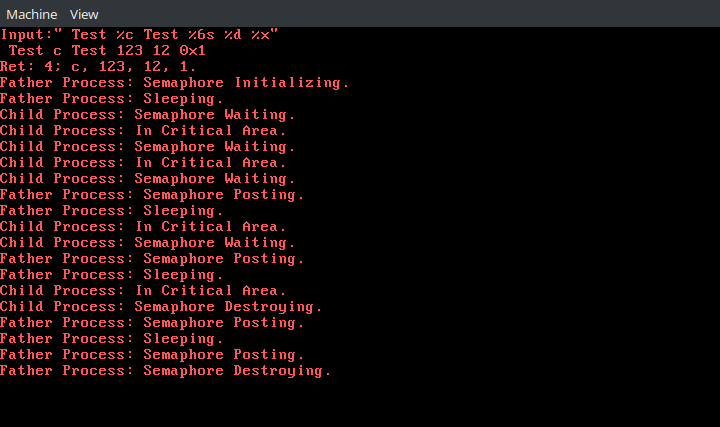
\includegraphics[width=\textwidth]{scanfsem}
	\caption{scanf和信号量运行结果}
\end{figure}

\subsection{哲学家问题}
\begin{figure}[htbp]
	\centering
	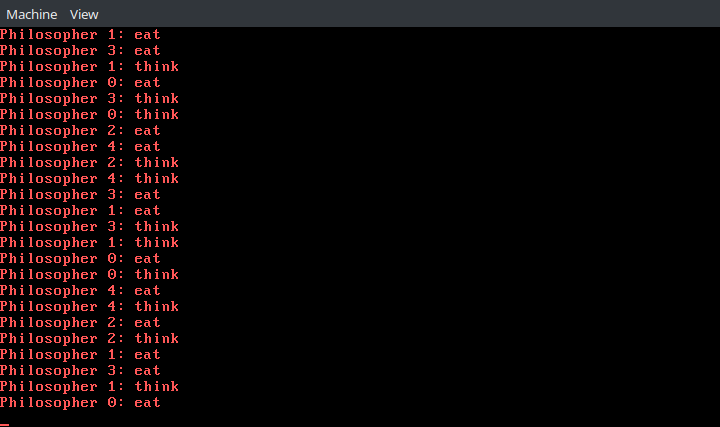
\includegraphics[width=\textwidth]{philosopher}
	\caption{哲学家问题结果}
\end{figure}

\newpage
\subsection{生产消费问题}
\begin{figure}[htbp]
	\centering
	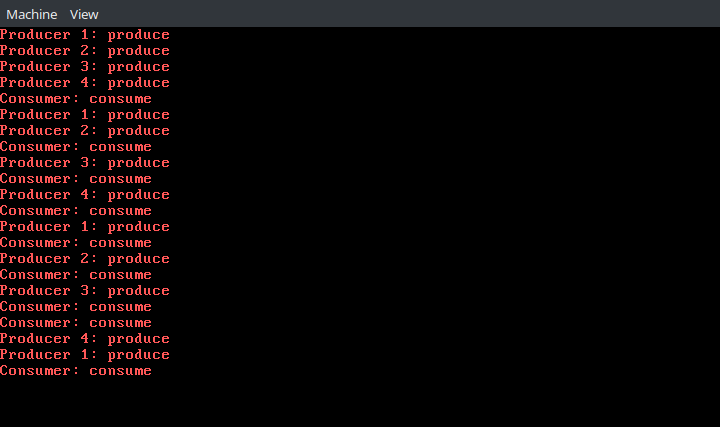
\includegraphics[width=\textwidth]{producer}
	\caption{生产消费问题运行结果}
\end{figure}

\newpage
\subsection{读写者问题}
\begin{figure}[htbp]
	\centering
	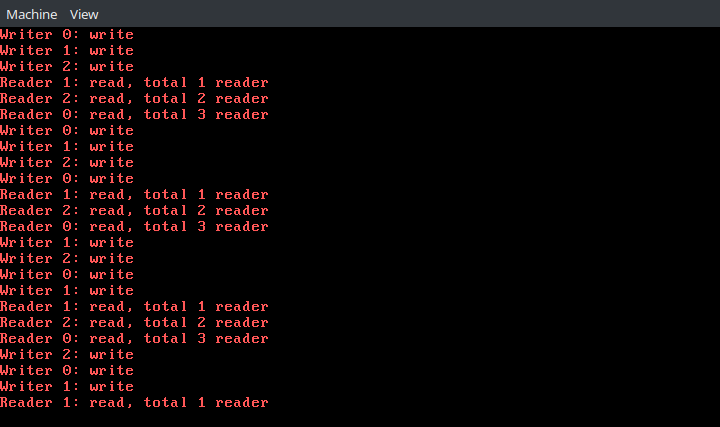
\includegraphics[width=\textwidth]{reader}
	\caption{读写者问题运行结果}
\end{figure}

\section{问题与思考}
\begin{enumerate}
	\item 在命令行中运行qemu-system-i386 os.img,窗口显示"no bootable device"。原因可能是gcc版本问题。安装gcc6并编译可成功运行。另外,还有一个解决方案是加一个编译参数-fno-asynchronous-unwind-tables,经过尝试也可以成功。查询相关资料知,"This option determines whether unwind information is precise at an instruction boundary or at a call boundary. If -fno-asynchronous-unwind-tables is specified, the unwind table is precise at call boundaries only."新版本的gcc默认行为是"-fasynchronous-unwind-tables",而旧版的gcc默认"-fno-asynchronous-unwind-tables"。猜想unwind information的位置不同将影响加载过程,而qemu模拟的是老式的硬件,可能会产生不匹配。
	\item 一开始写哲学家问题时总是出现fork返回-1的情况,经过很长时间的检查才发现框架代码默认只支持4个用户进程。修改NR\_SEGMENT可以改变最大进程数,才能正确运行。
\end{enumerate}

\section{建议}
\begin{enumerate}
	\item 建议将官方的实验环境升级到20.04LTS版本,这样不容易产生gcc版本问题,可以节省很多时间;
	\item 建议将memery.h中的NR\_SEGMENT直接修改为20。
\end{enumerate}

\end{document}